%%%%%%%%%%%%%%%%%%%%%%%%%%%%%%%%%%%%%%%%%%%%%%%%%%%%%%%%%%%%%%%%%%%%%%%%%%%%%%%%
%2345678901234567890123456789012345678901234567890123456789012345678901234567890
%        1         2         3         4         5         6         7         8

\documentclass[letterpaper, 10 pt, conference]{ieeeconf}  % Comment this line out if you need a4paper

%\documentclass[a4paper, 10pt, conference]{ieeeconf}      % Use this line for a4 paper

\IEEEoverridecommandlockouts   
\usepackage{graphicx}
\usepackage{amssymb}
\usepackage{amsmath}
\usepackage{changes}
\usepackage{xcolor}
\usepackage{colortbl}
\usepackage[table]{xcolor}
\usepackage{booktabs}

\newcommand{\EditSS}[1]{{\color{violet} #1}}
\newcommand{\EditAN}[1]{{\color{blue} #1}}

\usepackage[
backend=biber,
style=numeric,
sorting=none
]{biblatex}

\addbibresource{references.bib}

% This command is only needed if 
                                                          % you want to use the \thanks command

\overrideIEEEmargins                                      % Needed to meet printer requirements.

%In case you encounter the following error:
%Error 1010 The PDF file may be corrupt (unable to open PDF file) OR
%Error 1000 An error occurred while parsing a contents stream. Unable to analyze the PDF file.
%This is a known problem with pdfLaTeX conversion filter. The file cannot be opened with acrobat reader
%Please use one of the alternatives below to circumvent this error by uncommenting one or the other
%\pdfobjcompresslevel=0
%\pdfminorversion=4

% See the \addtolength command later in the file to balance the column lengths
% on the last page of the document

% The following packages can be found on http:\\www.ctan.org
%\usepackage{graphics} % for pdf, bitmapped graphics files
%\usepackage{epsfig} % for postscript graphics files
%\usepackage{mathptmx} % assumes new font selection scheme installed
%\usepackage{times} % assumes new font selection scheme installed
%\usepackage{amsmath} % assumes amsmath package installed
%\usepackage{amssymb}  % assumes amsmath package installed

\title{\LARGE \bf
Belief-aware VLM model for human-like Reasoning 
}


\author{Anshul Nayak$^{1}$, Shahil Shaik and Yue Wang$^{2}$% <-this % stops a space
\thanks{*Equal Contribution}% <-this % stops a space
\thanks{$^{1}$Albert Author is with Faculty of Electrical Engineering, Mathematics and Computer Science,
        University of Twente, 7500 AE Enschede, The Netherlands
        {\tt\small albert.author@papercept.net}}%
\thanks{$^{2}$Bernard D. Researcheris with the Department of Electrical Engineering, Wright State University,
        Dayton, OH 45435, USA
        {\tt\small b.d.researcher@ieee.org}}%
}

\begin{document}



\maketitle
\thispagestyle{empty}
\pagestyle{empty}


%%%%%%%%%%%%%%%%%%%%%%%%%%%%%%%%%%%%%%%%%%%%%%%%%%%%%%%%%%%%%%%%%%%%%%%%%%%%%%%%
\begin{abstract}

Traditional neural network models for intent inference rely heavily on observable states and struggle to generalize across diverse tasks and dynamic environments. Recent advances in Vision–Language Models (VLMs) and Vision–Language–Action (VLA) models introduce common-sense reasoning through large-scale multimodal pretraining, enabling zero-shot performance across tasks. However, these models still lack explicit mechanisms to represent and update belief, limiting their ability to reason like humans  or capture the  evolving human intent over long-horizon. To address this, we propose a belief-aware VLM framework that integrates retrieval-based memory and reinforcement learning. Instead of learning an explicit belief model, we approximate belief using a vector-based memory that retrieves relevant multimodal context, which is incorporated into the VLM for reasoning. We further refine decision-making using a reinforcement learning policy over the VLM latent space. We evaluate our approach on publicly available VQA datasets such as HD-EPIC and demonstrate consistent improvements over zero-shot baselines, highlighting the importance of belief-aware reasoning.

\end{abstract}


%%%%%%%%%%%%%%%%%%%%%%%%%%%%%%%%%%%%%%%%%%%%%%%%%%%%%%%%%%%%%%%%%%%%%%%%%%%%%%%%
\section{INTRODUCTION}




Robotic systems operating in human-centric environments must reason under uncertainty, anticipate future actions, and adapt to partially observable and dynamically evolving contexts. Classical frameworks for such decision-making—rooted in structured formulations such as Markov Decision Processes (MDPs) \cite{} and Partially Observable MDPs (POMDPs) \cite{} —explicitly model latent states and belief updates, enabling principled reasoning about uncertainty. These approaches have also inspired cognitive models of human reasoning, where agents maintain and update beliefs about other agents’ intents to guide decision-making \cite{}. Such belief-driven reasoning is fundamental in both human–human and human–robot interactions, where actions are not only conditioned on the physical state of the environment but also on inferred intentions, expectations, and uncertainties about others' belief.

Despite their theoretical rigor, traditional cognitive and probabilistic models \cite{} often rely on hand-crafted representations and simplifying assumptions that limit scalability in high-dimensional, multimodal environments. In parallel, modern deep learning approaches—particularly standard neural networks \cite{} trained end-to-end on visual or sequential data—have demonstrated strong perceptual capabilities but often lack explicit mechanisms for structured reasoning or belief modeling. As a result, existing intent inference methods are often limited by their reliance on observable states, lack of long-horizon reasoning, and poor generalization across tasks, particularly in complex multi-agent settings.

Recently, Vision–Language Models (VLMs)  have emerged as powerful general-purpose reasoning systems that integrate visual perception with semantic and contextual understanding \cite{}. Unlike conventional neural networks, VLMs leverage large-scale pretraining on diverse multimodal data, enabling zero-shot and few-shot generalization across a wide range of tasks. Their ability to jointly reason over visual inputs and language allows them to infer high-level semantics, contextual relationships, and implicit goals directly from raw observations. This makes VLMs particularly promising for modeling human behavior, where reasoning often involves interpreting both observable actions and latent intent.

However, directly applying VLMs in a zero-shot manner is insufficient for modeling nuanced human decision-making in interactive settings. Human behavior and decision-making is inherently belief-driven; individuals continuously update their beliefs about other agents based on observations and use these beliefs to guide their actions. Prior work in cognitive science and robotics has demonstrated the importance of such belief modeling for tasks including intention inference \cite{}, theory of mind \cite{}, and collaborative planning. Yet, existing VLM-based approaches largely overlook this aspect, treating reasoning as a static mapping from observations to actions without explicitly modeling the underlying belief dynamics to achieve human-like reasoning.

To address this limitation, we propose a \textbf{belief-aware Vision–Language Model (VLM)} that explicitly integrates belief dynamics into multimodal reasoning. Our key idea is to augment VLMs with a structured belief representation that captures an agent’s evolving estimate of other agents’ intents. Specifically, we model human decision-making as a belief-conditioned process, where actions are generated based not only on current observations but also on prior beliefs updated through interaction. In the current work, instead of learning an explicit parametric belief model, we construct a vector-based belief memory \cite{} that stores multimodal embeddings of past visual and textual contexts. Given a new observation, the model retrieves the top-K most relevant embeddings based on similarity, which serve as prior belief. This design allows the model to approximate belief updates through retrieval, avoiding the need for explicitly modeling belief dynamics while still capturing context-dependent reasoning.

% we move beyond zero-shot inference by fine-tuning the VLM for belief-conditioned reasoning through a combination of parameter-efficient adaptation and reinforcement learning.

Crucially,  the  belief mechanism provides prior contextual information grounded in concrete situational understanding and when combined with multimodal inputs, it enables the VLM to form a richer representation of the environment and agent intent. VLMs generate outputs based on these learned contextual patterns and may lack consistency and goal-directed behavior in decision-making. To address this, we pass the latent representation of the VLM to a reinforcement learning policy, which refines action selection by optimizing task-specific rewards using policy gradient methods. In this framework, belief enhances the quality of reasoning, while RL ensures that the resulting decisions are optimized with respect to task objectives. Many publicly available vision-question answering (VQA) datasets  such as EPIC-Kitchens, NExT-QA, and HD-EPIC \cite{}, can be utilized to  demonstrate current model's performance over zero-shot baselines, highlighting the effectiveness of combining belief-aware representations with reward-driven reasoning.


Our key contributions are summarized as follows:

\begin{itemize}

\item 
We propose a novel \textbf{Belief-aware VLM} framework that incorporates belief into Vision--Language Models through a vector-based memory, where relevant prior multimodal embeddings are retrieved using similarity search to approximate latent belief without requiring an explicit parametric belief model. This enables the VLM to perform context-aware reasoning and approximate intent inference in human--robot interaction settings.



\item We propose a hybrid fine-tuning method that  
combines parameter-efficient fine-tuning (PEFT) methods such as LoRA for efficient adaptation of belief-aware representations while reinforcement learning refines decision-making and reasoning through reward-driven optimization.


\item We evaluate our model on popular Vision Query Answer (VQA) datasets such as HD-EPIC \cite{11094504} and show improvement over zero-shot inference performance using state-of-the-art VLMS and other baselines.   


\end{itemize}


\section{Related Work}

\subsection{Intent Modeling}

Understanding human preferences and intentions in human–robot collaboration is critical for effective task execution, transparency, and trust. Prior work has approached intent inference using probabilistic and learning-based methods, including Hidden Markov Models (HMMs) \cite{PETKOVIC2019182} and Dynamic Bayesian Networks (DBNs) \cite{xu2015optimo, hao2025joint} for modeling temporal dependencies, as well as Partially Observable Markov Decision Processes (POMDPs) \cite{zhao2022coordination, bai2015intention} for belief-based reasoning under uncertainty. Supervised approaches, such as Support Vector Machines (SVMs) \cite{kang2015human} and Neural Networks (NNs) \cite{hu2022augmented}, have also been used to predict intent directly from observed features.

Despite their success, these methods often rely on observable states and struggle to generalize across diverse tasks and environments. They are limited by insufficient world knowledge, weak incorporation of language and contextual cues, and short context horizons that hinder modeling of long-term dependencies and evolving goals. These challenges are further amplified in multi-human, multi-robot settings, where systems must reason over multiple, potentially conflicting intentions and operate within a rapidly expanding state–action space.



\subsection{Cognitive Modeling With LLM}
Recent advances in Vision–Language Models (VLMs) and Vision–Language–Action (VLA) models have enabled strong zero-shot reasoning by leveraging large-scale multimodal pretraining. Models such as PaLM-E \cite{driess2023palm} and RT-2 \cite{brohan2023rt2visionlanguageactionmodelstransfer} demonstrate that grounding language in perception allows reasoning over physical environments and actions. However, despite exhibiting elements of common-sense reasoning, these approaches lack explicit mechanisms to model belief, intent, and evolving context, limiting their ability to capture long-horizon dependencies and dynamic interactions.

In contrast, cognitive models explicitly incorporate latent belief and intent. Early work on Theory of Mind (ToM) \cite{pmlr-v80-rabinowitz18a} introduced architectures for inferring hidden mental states, while recent studies \cite{zhu2024language} show that LLMs implicitly encode belief representations in their internal activations. Additional efforts integrating cognitive frameworks with LLMs \cite{wu2024cognitive} and alignment methods such as RLHF \cite{havrilla2024teaching} further improve reasoning consistency, highlighting the importance of structured, belief-aware representations for human-like reasoning.
% Despite these developments, most LLM and VLM approaches still do not explicitly model belief dynamics, which are central to human cognition. Bridging this gap requires integrating structured belief representations with multimodal reasoning. In this work, we address this limitation by incorporating belief-aware reasoning into a VLM framework and refining decision-making through reinforcement learning, enabling more human-like inference grounded in both perception and interaction.
%{Alternatively, VLMs can understand multi-modal context to capture underlying features and predict human intent. }  %\added{[Is this the same for VLM i.e uncertainty in inferring intent?]}. 
%\EditAAN{Both VLM and traditional methods are susecptible to uncertainty. In fact, POMDPs and DBNs can be helpful in quantifying uncertainty to some degree while VLMs hallucinate and may overestimate or underestimate their reasoning ability. I believe the VLMs generally shine at generalizing across different tasks and learning } 


\subsection{RL for LLM reasoning}

Building on these limitations, adapting large VLMs and LLMs to human–robot interaction requires both efficient model adaptation and improved decision-making. Parameter-efficient fine-tuning (PEFT) methods \cite{ding2023parameter, hu2022lora} address scalability by updating only a small subset of parameters while keeping the pretrained backbone fixed, enabling efficient alignment of multimodal representations with task-specific inputs. However, while PEFT improves representation learning, it does not explicitly optimize reasoning or action selection.

To address this, reinforcement learning (RL) has been used to refine model outputs by optimizing task-specific rewards. Approaches such as reinforcement learning from AI feedback (RLAIF) \cite{lee2023rlaif}, improve reasoning by aligning model outputs with desired behaviors, including correctness, consistency, and task completion. This is particularly important in embodied settings, where reasoning must be grounded in both perception and action, motivating the integration of reward-driven optimization with multimodal reasoning models.



\begin{figure*}
    \centering  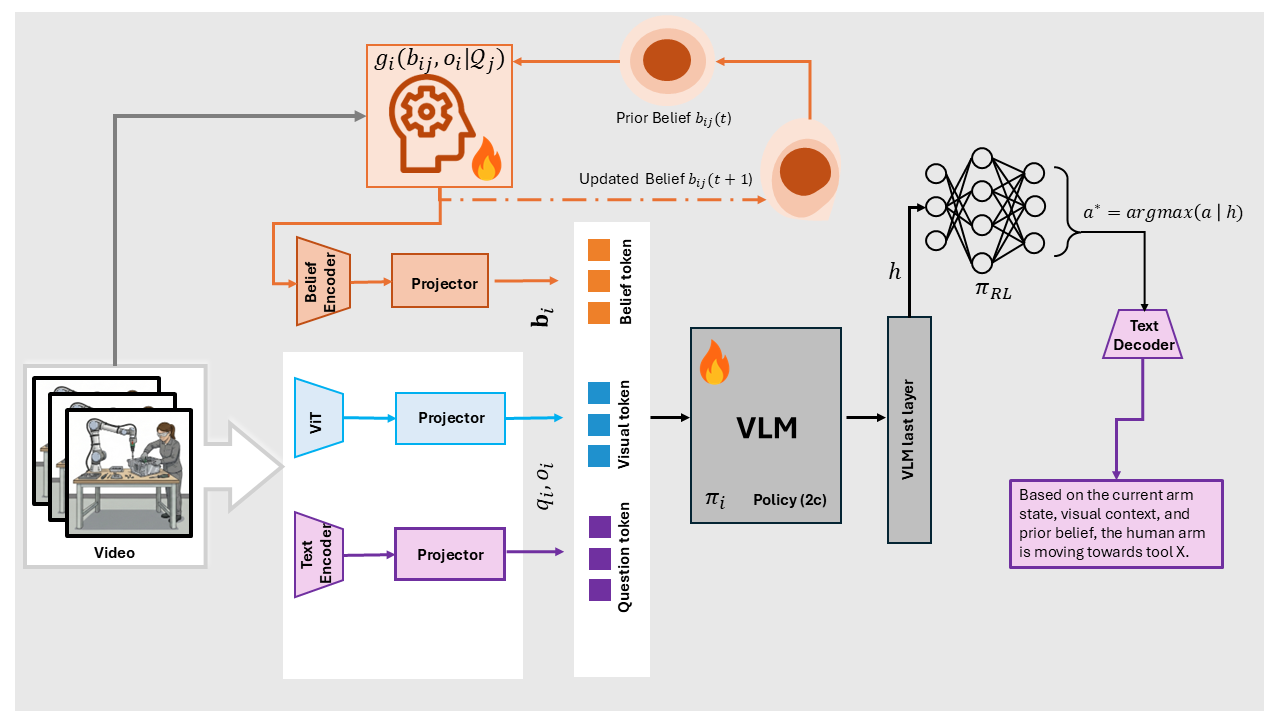
\includegraphics[width=1.0\linewidth]{Architecture_ROMAN.png}
    \caption{Caption}
    \label{fig:placeholder}
\end{figure*}


% \subsection{Belief MDP Formulation}

% We formulate the interaction as a belief MDP, where the belief summarizes past observations and evolves recursively. The classical Bayesian update is given by:
% \begin{equation}
% b_{ij}(t+1)(q_j) \propto P(o_i(t+1) \mid q_j, a_j(t)) \cdot b_{ij}(t)(q_j)
% \end{equation}

% However, explicitly modeling the observation likelihood is intractable for high-dimensional inputs such as video and language. Therefore, we approximate belief updates using a learned model:
% \begin{equation}
% b_{ij}(t+1) = g_\psi\big(b_{ij}(t), a_j(t), o_i(t+1)\big)
% \end{equation}

% We further model the coupled belief and decision-making process for a human--robot pair as:


% where $x_i(t)$ denotes the human state, $a_i(t)$ the human action, and $b_{ij}(t)$ the belief of human $i$ about agent $j$'s intent. The policy $\pi_i$ is conditioned on both the current state and the belief over other agents.

\EditSS{
\section{Preliminaries}
We first introduce the three main components of our framework: a retrieval-based prior belief memory, a vision--language model (VLM) for multimodal context encoding, and a reinforcement learning (RL) policy for answer selection. Let a video clip be denoted by $v$, a natural-language question by $q$, and a set of answer candidates by $\mathcal{A} = \{a_1, \dots, a_K\}$. The goal is to predict the correct answer index $y \in \{1, \dots, K\}$ in a way that is consistent with human intent.

Overall, the framework operates as follows: a prior belief prompt $b$ is first retrieved from an external memory bank, the VLM then encodes the multimodal input $(v, q, \mathcal{A}, b)$ into a latent state $h$, and a lightweight policy head predicts the final answer based on $h$.

\subsection{Multimodal Context Encoding}
Given the current video clip, question, answer candidates, and an optional prior belief prompt, a pretrained VLM maps the multimodal context into a fused latent representation:
\begin{equation}
h = f_{\theta}(v, q, \mathcal{A}, b),
\end{equation}
where $b$ denotes the retrieved prior belief prompt and $\theta$ denotes the VLM parameters. In our framework, the VLM serves as a multimodal context encoder that transforms visual and textual inputs into a shared latent state suitable for downstream decision-making. Depending on the training configuration, the VLM may be frozen, fine-tuned using LoRA, or fully fine-tuned.

\subsection{Retrieval-Based Prior Belief}
Rather than explicitly learning belief dynamics, we maintain an external memory bank
\begin{equation}
\mathcal{M} = \{(m_k, c_k)\}_{k=1}^{N},
\end{equation}
where $m_k$ is the embedding of a past observation and $c_k$ is the associated contextual text stored in memory. Given a current query embedding $u$, we retrieve the top-$K$ nearest entries according to a similarity score:
\begin{equation}
\mathcal{N}_K(u) = \operatorname{TopK}_{k}\; \mathrm{sim}(u, m_k).
\end{equation}
The retrieved text snippets are then formatted into a prior belief prompt and prepended to the original question. In this way, the retrieved context serves as an approximate prior belief over latent task-relevant factors, allowing the model to reason using historically grounded contextual cues rather than relying solely on the current observation. In practice, the memory can be constructed either from text embeddings alone or from multimodal VLM embeddings, depending on the retrieval setting.

\subsection{Policy Over VLM States}
The fused latent state $h$ produced by the VLM is passed to a lightweight policy network
\begin{equation}
\pi_{\phi}(a \mid h),
\end{equation}
where $\phi$ denotes the policy parameters. The policy outputs a distribution over answer candidates and acts as a human-like decision module on top of the VLM representation. In the PPO-based setting, the policy is optimized using a scalar reward derived from answer correctness.

For multiple-choice VQA, we define the reward as
\begin{equation}
r(h,a) =
\begin{cases}
1, & \text{if } \hat{y} = y,\\
0, & \text{otherwise}.
\end{cases}
\end{equation}
The policy objective is to maximize the expected reward:
\begin{equation}
J(\pi_{\phi}) = \mathbb{E}_{\pi_{\phi}} \left[ r(h,a) \right].
\end{equation}
Using the policy gradient theorem, the gradient of this objective can be written as
\begin{equation}
\nabla_{\phi} J(\pi_{\phi})
=
\mathbb{E}_{\pi_{\phi}} \left[
\nabla_{\phi} \log \pi_{\phi}(a \mid h)\,
A^{\pi_{\phi}}(h,a)
\right],
\end{equation}
where $A^{\pi_{\phi}}(h,a)$ denotes the advantage function. When the VLM is trainable, supervised cross-entropy loss on the ground-truth answer can be combined with the policy objective to stabilize learning and improve sample efficiency.
}

\section{Methodology}

\subsection{Preliminaries}

We begin by establishing necessary background in the section. 
 Let $o_t \in \mathbf{\mathcal{O}}$ denote observations and $s_t \in \mathcal{S}$ denote latent states; the agent maintains an implicit belief $b_{i}$ over latent variables conditioned on the observation history. Latent embeddings and  learning representations are presented as $z = {\phi}(o_t) \in \mathbb{R}^d$, where heterogeneous inputs such as vision and language are embedded into a shared latent space that captures semantic and contextual information. Prior belief is incorporated using retrieval-based mechanisms which augment neural models with an external memory $\mathcal{M} = \{z_k\}_{k=1}^N$, where relevant contexts are selected using a similarity function $\text{sim}(z_t, z_k)$, enabling conditioning on past observations without explicitly modeling belief dynamics. For decision-making, policies $\pi_{RL}(a_t \mid z_t)$ are optimized using reinforcement learning, where the objective is to maximize expected cumulative reward $J(\pi) = \mathbb{E}_{\pi} \left[ \sum_{t=0}^{\infty} \gamma^t R(s_t, a_t) \right]$. Policy optimization is typically performed via gradient-based methods that update parameters in the direction of expected return, such as $\nabla_{\theta} J(\pi) = \mathbb{E}_{\pi} \left[ \nabla_{\theta} \log \pi_{\theta}(a_t \mid z_t) Q^{\pi}(z_t, a_t) \right]$. These components namely the latent representation learning, retrieval-augmented context modeling, and reward-driven policy optimization form the foundation for reasoning and decision-making in high-dimensional, partially observable environments.

\subsection{Problem Formulation}

We formulate our problem under partial observability, where an  agent $i$ must reason the latent intent of another agent $j$ (robot or human) from multi-modal observations. The interaction evolves over time, where at each time step $t$, the agent observes
$o_i(t) = \{v(t), \ell(t)\}$
where $v(t)$ denotes visual observations and $\ell(t)$ denotes contextual language inferred from the scene. 
We assume that the intent $q_j \in \mathcal{Q}_j$ for the agent, evolves on a \emph{slow time-scale} and remains constant during human-robot sensorimotor interaction. $\mathcal{Q}_{j}$ represents set of all possible intents for agent j.
\begin{equation}
q_j(\tau + 1) \approx q_j(\tau), \quad \forall t \in [\tau, \tau + \Delta T]
\end{equation}
% This assumption allows us to decouple high-frequency motion dynamics from low-frequency intent reasoning, focusing on belief inference over intent rather than instantaneous motion prediction.
 
 Since the intent $q_j$ of agent $j$ is latent and not directly observable, agent $i$ maintains a belief distribution $b_{ij}$  over $q_{j}$.
\begin{equation}
b_{ij}(t+1) = {P}(b_{ij}(t), o_{i}(t) \mid q_{j})
\end{equation}

The  belief distribution evolves temporally $b_{ij}(t + 1)$ based on agent i’s prior belief $b_{ij}(t)$ of other agent's 
intent and the observation.
% The belief evolves as new observations are received and serves as a sufficient statistic for decision-making under partial observability.
The multimodal observation $o_{i}(t)$ is  processed through a pretrained encoder  to create latent embedding, $
z(t) =\phi(v(t), \ell(t))$. The embedding $z(t)$ along with belief $b_{ij}(t)$ is then projected  as inputs to a Vision Language Model (VLM) $\pi_{i}^{\theta}$. 
% The belief-aware VLM is parameterized by $\theta$, which produces a contextualized representation of the task provided prior belief and can be learned  in an end-to-end fashion using a total loss function that couples  action and belief estimation $\mathcal{L}= 
%     \mathcal{L}_{a}+
%     \mathcal{L}_{b}$. Model training is achieved by either full fine-tuning of the parameters $\theta$ or using PEFT  methods.  In a supervised setting, the belief loss $\mathcal{L}_b$ directly compares the output of $g_i$ by minimizing the prediction $\tilde{b}_{ij}(t+1:t+T)$ and the ground truth $b_{ij}(t+1:t+T)$. However,  the current approach does not train the belief model $g_{i}$ rather it stores the vision-language contextual embeddings in a vector database and builds a prior belief based on top-K features when queried.
The belief-aware VLM, parameterized by $\theta$, produces a contextualized representation of the task conditioned on multimodal observations and prior belief. The model can be trained end-to-end using a joint objective that couples action prediction and belief alignment, given by $\mathcal{L} = \mathcal{L}_a + \mathcal{L}_b$. Training can be performed either via full fine-tuning of $\theta$ or through parameter-efficient fine-tuning (PEFT) methods.

In a supervised setting, the belief loss $\mathcal{L}_b$ directly compares the output of $g_i$ by minimizing the prediction $\tilde{b}_{ij}(t+1:t+T)$ and the ground truth $b_{ij}(t+1:t+T)$.
Unlike prior approaches that explicitly learn a belief model $g_i$, our formulation does not parameterize belief dynamics. Instead, we maintain a vector-based memory of vision--language embeddings and approximate prior belief by retrieving the top-$K$ most relevant contexts based on similarity. 
\paragraph{Belief from Top-$K$ Retrieval}
 Given the current embedding $z(t)$, we retrieve the top-$K$ most similar entries:
\begin{equation}
\mathcal{N}_K(z(t)) = \text{TopK}_k \; \text{sim}(z(t), z_k),
\end{equation}
where $\text{sim}(\cdot,\cdot)$ denotes a similarity function (e.g., cosine similarity). The belief is then computed as a similarity-weighted aggregation:
\begin{align}
b_{ij}(t) &= \sum_{k \in \mathcal{N}_K(z(t))} w_k \, c_k, \\ \nonumber
w_k &= \frac{\exp(\text{sim}(z(t), z_k))}{\sum_{j \in \mathcal{N}_K(z(t))} \exp(\text{sim}(z(t), z_j))}.
\end{align}
where $c_k$ represents the contextual embedding associated with memory entry $z_k$. This retrieval mechanism provides an implicit belief representation without requiring direct supervision. $h(t)$  encodes inferred intent and relevant prior knowledge which helps capture task-specific contextual information  and serves as the latent state for downstream action selection. 
\begin{equation}
h(t) = \pi_{i}^{\theta}(z(t), b_{ij}(t))
\end{equation}
 

Typically, action selection is modeled as a direct mapping from observations and prior belief to actions:
\begin{equation}
a_i(t) \sim \pi_i(o_{i}(t), b_{ij}(t))
\end{equation}

While this formulation enables belief-aware decision-making, it does not explicitly optimize actions for task-specific objectives, often leading to suboptimal performance. To address this, we refine the policy using reinforcement learning to directly optimize action selection based on task-specific rewards.
% \textbf{Belief Inference via VLM.}  
% From the latent representation, we infer a belief distribution over possible intents:
% \begin{equation}
% \hat{b}_{ij}(t) = \text{softmax}(W_b h(t))
% \end{equation}

% Thus, the VLM serves as a belief inference model:
% \begin{equation}
% \hat{b}_{ij}(t) \approx P(q_j \mid z(t))
% \end{equation}
 


\subsection{Reinforcement Learning Fine-Tuning of VLM Policy}

The final layer of the VLM produces a contextual representation $h(t)$ that encodes multimodal observations, inferred belief, and task-relevant semantics. While $h(t)$ captures rich reasoning, it does not explicitly optimize decision-making for task-specific objectives. To address this, we introduce a reinforcement learning (RL) policy that operates on top of the VLM representation.

\medskip

\noindent
\textbf{RL Policy over VLM Representation.}  
We define a policy $\pi_{\text{RL}}$ that maps the latent representation $h(t)$ to a distribution over actions:
\begin{equation}
\pi_{\text{RL}}(\hat{a} \mid h(t)) = \text{NN}_{\phi}(h(t)),
\end{equation}
where $\phi$ denotes the parameters of a lightweight policy network.

\medskip

\noindent
\textbf{Utility-Based Decision Making.}  
The action selection process is guided by a utility function:
\begin{equation}
U_i(x_i(t), q_i(\tau), x_{\mathcal{N}_i}(t)) \in \mathbb{R},
\end{equation}
where $x_i(t)$ denotes the agent state, $q_i(\tau)$ the latent intent, and $x_{\mathcal{N}_i}(t)$ the states of neighboring agents. The inferred belief influences the expected utility over actions.

\medskip

\noindent
\textbf{Reward and Action Selection.}  
We interpret the reward as a realization of utility, i.e., $R(a) \equiv U_i(\cdot)$, and select actions by maximizing expected reward:
\begin{equation}
a^* = \arg\max_{a \in \mathcal{A}} \mathbb{E}[R(a \mid h(t))].
\end{equation}

\medskip

\noindent
\textbf{Policy Optimization.}  
The policy is optimized to maximize expected cumulative reward:
\begin{equation}
J(\pi_{\text{RL}}) = \mathbb{E}_{\pi_{\text{RL}}} \left[ \sum_{t} \gamma^t R(a_t) \right].
\end{equation}
Gradients are computed using policy gradient methods and propagated through the policy network, and optionally into the VLM enabling improved reasoning and action selection.

% \medskip

% \noindent
% \textbf{Utility-Based Interpretation.}  
% The decision process can be interpreted as maximizing a utility function:
% \begin{equation}
% U_i(x_i(t), q_i(\tau), x_{\mathcal{N}_i}(t)) \in \mathbb{R}
% \end{equation}

% where $x_i(t)$ denotes the agent state and $x_{\mathcal{N}_i}(t)$ represents neighboring agents. The inferred belief influences the expected utility over actions.



% While the VLM provides a strong prior for reasoning and belief inference, it is not explicitly optimized for task-specific decision-making. To address this, we introduce a reinforcement learning (RL) policy that operates on top of the VLM representation.

% \medskip

% \noindent
% \textbf{RL Policy over VLM Representation.}  
% We define a policy $\pi_{\text{RL}}$ that maps the latent representation $h(t)$ to a distribution over actions:
% \begin{equation}
% \pi_{\text{RL}}(\hat{a} \mid h(t)) = \text{NN}_{\phi}(h(t))
% \end{equation}

% where $\phi$ denotes trainable parameters of a lightweight neural policy head.

% \medskip

% \noindent
% \textbf{Action Selection.}  
% The optimal action is selected by maximizing expected reward:
% \begin{equation}
% a^* = \arg\max_{a \in \mathcal{A}} \mathbb{E}[R(a \mid h(t))]
% \end{equation}

% where $R$ is a scalar reward function defined over candidate actions or options.

% \medskip

% \noindent
% \textbf{Reward Utility.}  
% The reward can be interpreted as a utility function over actions:
% \begin{equation}
% R(a) \equiv U_i(x_i(t), q_i(\tau), x_{\mathcal{N}_i}(t))
% \end{equation}

% linking the RL objective with the underlying belief-conditioned decision-making process.

% \medskip

% \noindent
% \textbf{Policy Optimization.}  
% The RL policy is optimized to maximize expected cumulative reward:
% \begin{equation}
% J(\pi_{\text{RL}}) = \mathbb{E}_{\pi_{\text{RL}}} \left[ \sum_{t} \gamma^t R(a_t) \right]
% \end{equation}

% Gradients are propagated through the policy head and optionally into the VLM via parameter-efficient fine-tuning (PEFT), such as LoRA.

% \medskip

% \noindent
% \textbf{Role of VLM in RL Loop.}  
% In this framework:
% \begin{itemize}
%     \item The VLM provides a structured latent representation $h(t)$ encoding belief and context
%     \item The RL policy $\pi_{\text{RL}}$ optimizes decision-making over this representation
% \end{itemize}

% This separation allows the model to retain the generalization capabilities of pretrained VLMs while adapting decision-making through reward-driven learning.

% \medskip

% \noindent
% \textbf{Key Insight.}  
% The overall pipeline can be summarized as:
% \begin{equation}
% (v, \ell) \rightarrow z \rightarrow h \rightarrow \{b, a\}
% \end{equation}

% where belief is inferred from $h$, and actions are optimized via RL. This transforms the VLM from a passive reasoning model into a belief-aware decision-making system.



\section{EXPERIMENTS}


\subsection{Multi-modal Representation learning}



\subsection{Belief Model}


\begin{table}[t]
\centering
\scriptsize
\setlength{\tabcolsep}{2.5pt}   % reduce column spacing
\renewcommand{\arraystretch}{1.05}

\resizebox{\columnwidth}{!}{ % ensures it fits ONE column
\begin{tabular}{lcccccccc}
\toprule
\textbf{Model} & 
\cellcolor{red!20}\textbf{Recipe} & 
\cellcolor{orange!25}\textbf{Ingredient} & 
\cellcolor{yellow!30}\textbf{Nutrition} & 
\cellcolor{green!25}\textbf{Action} & 
\cellcolor{blue!20}\textbf{3D} & 
\cellcolor{cyan!20}\textbf{Motion} & 
\cellcolor{magenta!20}\textbf{Gaze} & 
\textbf{Avg.} \\
\midrule

\multicolumn{9}{l}{\textbf{Blind - Language Only}} \\
Llama 3.2 & 33.5 & 25.0 & 36.7 & 23.3 & 22.3 & 25.5 & 19.5 & 26.5 \\
Gemini Pro & 38.0 & 26.8 & 30.0 & 22.1 & 21.5 & 27.7 & 20.5 & 26.7 \\

\midrule
\multicolumn{9}{l}{\textbf{Video-Language}} \\
VideoLlama 2 & 30.8 & 25.7 & 32.7 & 27.2 & 25.7 & 28.5 & 21.2 & 27.4 \\
LongVA & 29.6 & 30.8 & 33.7 & 30.7 & 32.9 & 22.7 & 24.5 & 29.3 \\
LLaVA-Video & 36.3 & 33.5 & 38.7 & 43.0 & 27.3 & 18.9 & 29.3 & 32.4 \\
Gemini Pro & 60.5 & 46.2 & 34.7 & 39.6 & 32.5 & 20.8 & 28.7 & 37.6 \\

\midrule
\textit{Sample Human Baseline} & 96.7 & 96.7 & 85.0 & 92.5 & 93.8 & 92.7 & 75.0 & 90.3 \\
\bottomrule
\end{tabular}
}

\caption{\textbf{VQA Results per Category (\% Acc.).} Our benchmark remains challenging for state-of-the-art video VLM models.}
\label{tab:vqa_results}
\end{table}


\subsection{Equations}







\begin{table}[h]
\caption{An Example of a Table}
\label{table_example}
\begin{center}
\begin{tabular}{|c||c|}
\hline
One & Two\\
\hline
Three & Four\\
\hline
\end{tabular}
\end{center}
\end{table}


   \begin{figure}[thpb]
      \centering
      \framebox{\parbox{3in}{We suggest that you use a text box to insert a graphic (which is ideally a 300 dpi TIFF or EPS file, with all fonts embedded) because, in an document, this method is somewhat more stable than directly inserting a picture.
}}
      %\includegraphics[scale=1.0]{figurefile}
      \caption{Inductance of oscillation winding on amorphous
       magnetic core versus DC bias magnetic field}
      \label{figurelabel}
   \end{figure}
   



\section{CONCLUSIONS}

 

\addtolength{\textheight}{-2cm}   % This command serves to balance the column lengths
                                  % on the last page of the document manually. It shortens
                                  % the textheight of the last page by a suitable amount.
                                  % This command does not take effect until the next page
                                  % so it should come on the page before the last. Make
                                  % sure that you do not shorten the textheight too much.

%%%%%%%%%%%%%%%%%%%%%%%%%%%%%%%%%%%%%%%%%%%%%%%%%%%%%%%%%%%%%%%%%%%%%%%%%%%%%%%%



%%%%%%%%%%%%%%%%%%%%%%%%%%%%%%%%%%%%%%%%%%%%%%%%%%%%%%%%%%%%%%%%%%%%%%%%%%%%%%%%



%%%%%%%%%%%%%%%%%%%%%%%%%%%%%%%%%%%%%%%%%%%%%%%%%%%%%%%%%%%%%%%%%%%%%%%%%%%%%%%%
\section*{APPENDIX}

Appendixes should appear before the acknowledgment.

\section*{ACKNOWLEDGMENT}

The preferred spelling of the word ÒacknowledgmentÓ in America is without an ÒeÓ after the ÒgÓ. Avoid the stilted expression, ÒOne of us (R. B. G.) thanks . . .Ó  Instead, try ÒR. B. G. thanksÓ. Put sponsor acknowledgments in the unnumbered footnote on the first page.



%%%%%%%%%%%%%%%%%%%%%%%%%%%%%%%%%%%%%%%%%%%%%%%%%%%%%%%%%%%%%%%%%%%%%%%%%%%%%%%%

References are important to the reader; therefore, each citation must be complete and correct. If at all possible, references should be commonly available publications.


\printbibliography

% \begin{thebibliography}{99}

% \bibitem{c1} G. O. Young, ÒSynthetic structure of industrial plastics (Book style with paper title and editor),Ó 	in Plastics, 2nd ed. vol. 3, J. Peters, Ed.  New York: McGraw-Hill, 1964, pp. 15Ð64.
% \bibitem{c2} W.-K. Chen, Linear Networks and Systems (Book style).	Belmont, CA: Wadsworth, 1993, pp. 123Ð135.
% \bibitem{c3} H. Poor, An Introduction to Signal Detection and Estimation.   New York: Springer-Verlag, 1985, ch. 4.
% \bibitem{c4} B. Smith, ÒAn approach to graphs of linear forms (Unpublished work style),Ó unpublished.
% \bibitem{c5} E. H. Miller, ÒA note on reflector arrays (Periodical styleÑAccepted for publication),Ó IEEE Trans. Antennas Propagat., to be publised.
% \bibitem{c6} J. Wang, ÒFundamentals of erbium-doped fiber amplifiers arrays (Periodical styleÑSubmitted for publication),Ó IEEE J. Quantum Electron., submitted for publication.
% \bibitem{c7} C. J. Kaufman, Rocky Mountain Research Lab., Boulder, CO, private communication, May 1995.
% \bibitem{c8} Y. Yorozu, M. Hirano, K. Oka, and Y. Tagawa, ÒElectron spectroscopy studies on magneto-optical media and plastic substrate interfaces(Translation Journals style),Ó IEEE Transl. J. Magn.Jpn., vol. 2, Aug. 1987, pp. 740Ð741 [Dig. 9th Annu. Conf. Magnetics Japan, 1982, p. 301].
% \bibitem{c9} M. Young, The Techincal Writers Handbook.  Mill Valley, CA: University Science, 1989.
% \bibitem{c10} J. U. Duncombe, ÒInfrared navigationÑPart I: An assessment of feasibility (Periodical style),Ó IEEE Trans. Electron Devices, vol. ED-11, pp. 34Ð39, Jan. 1959.
% \bibitem{c11} S. Chen, B. Mulgrew, and P. M. Grant, ÒA clustering technique for digital communications channel equalization using radial basis function networks,Ó IEEE Trans. Neural Networks, vol. 4, pp. 570Ð578, July 1993.
% \bibitem{c12} R. W. Lucky, ÒAutomatic equalization for digital communication,Ó Bell Syst. Tech. J., vol. 44, no. 4, pp. 547Ð588, Apr. 1965.
% \bibitem{c13} S. P. Bingulac, ÒOn the compatibility of adaptive controllers (Published Conference Proceedings style),Ó in Proc. 4th Annu. Allerton Conf. Circuits and Systems Theory, New York, 1994, pp. 8Ð16.
% \bibitem{c14} G. R. Faulhaber, ÒDesign of service systems with priority reservation,Ó in Conf. Rec. 1995 IEEE Int. Conf. Communications, pp. 3Ð8.
% \bibitem{c15} W. D. Doyle, ÒMagnetization reversal in films with biaxial anisotropy,Ó in 1987 Proc. INTERMAG Conf., pp. 2.2-1Ð2.2-6.
% \bibitem{c16} G. W. Juette and L. E. Zeffanella, ÒRadio noise currents n short sections on bundle conductors (Presented Conference Paper style),Ó presented at the IEEE Summer power Meeting, Dallas, TX, June 22Ð27, 1990, Paper 90 SM 690-0 PWRS.
% \bibitem{c17} J. G. Kreifeldt, ÒAn analysis of surface-detected EMG as an amplitude-modulated noise,Ó presented at the 1989 Int. Conf. Medicine and Biological Engineering, Chicago, IL.
% \bibitem{c18} J. Williams, ÒNarrow-band analyzer (Thesis or Dissertation style),Ó Ph.D. dissertation, Dept. Elect. Eng., Harvard Univ., Cambridge, MA, 1993. 
% \bibitem{c19} N. Kawasaki, ÒParametric study of thermal and chemical nonequilibrium nozzle flow,Ó M.S. thesis, Dept. Electron. Eng., Osaka Univ., Osaka, Japan, 1993.
% \bibitem{c20} J. P. Wilkinson, ÒNonlinear resonant circuit devices (Patent style),Ó U.S. Patent 3 624 12, July 16, 1990. 








\end{document}
